\documentclass[a4paper,14pt,oneside,final]{extarticle}
\usepackage[top=2cm, bottom=2cm, left=3cm, right=1cm]{geometry}
\usepackage{scrextend}

\usepackage[T2A,T1]{fontenc}
\usepackage[ukrainian,russian,english]{babel}
\usepackage{tempora}
\usepackage{fontspec}
\setmainfont{tempora}

% Зачем: Отключает использование изменяемых межсловных пробелов.
% Почему: Так не принято делать в текстах на русском языке.
\frenchspacing

\usepackage{indentfirst}
\setlength{\parindent}{1.25cm}
\renewcommand{\baselinestretch}{1.5}

% Header
\usepackage{fancyhdr}
\pagestyle{fancy}
\fancyhead{}
\fancyfoot{}
\fancyhead[R]{\small \selectfont \thepage}
\renewcommand{\headrulewidth}{0pt}

% Captions
\usepackage{chngcntr}
\counterwithin{figure}{section}
\counterwithin{table}{section}
\usepackage[tableposition=top]{caption}
\usepackage{subcaption}
\DeclareCaptionLabelFormat{gostfigure}{Рисунок #2}
\DeclareCaptionLabelFormat{gosttable}{Таблиця #2}
\DeclareCaptionLabelSeparator{gost}{~---~}
\captionsetup{labelsep=gost}
\captionsetup[figure]{labelformat=gostfigure}
\captionsetup[table]{labelformat=gosttable}
\renewcommand{\thesubfigure}{\asbuk{subfigure}}

% Sections
\usepackage[explicit]{titlesec}
\newcommand{\sectionbreak}{\clearpage}

\titleformat{\section}
  {\centering}{\thesection \quad}{0pt}{\MakeUppercase{#1}}
\titleformat{\subsection}[block]
  {\bfseries}{\thesubsection \quad #1}{0cm}{}

\titlespacing{\section} {0cm}{0cm}{21pt}
\titlespacing{\subsection} {\parindent}{21pt}{0cm}
\titlespacing{\subsubsection} {\parindent}{0cm}{0cm}

% Lists
\usepackage{enumitem}
\renewcommand\labelitemi{--}
\setlist[itemize]{noitemsep, topsep=0pt, wide}
\setlist[enumerate]{noitemsep, topsep=0pt, wide, label=\arabic*}
\setlist[description]{labelsep=0pt, noitemsep, topsep=0pt, leftmargin=2\parindent, labelindent=\parindent, labelwidth=\parindent, font=\normalfont}

% Toc
\usepackage{tocloft}
\tocloftpagestyle{fancy}
\renewcommand{\cfttoctitlefont}{}
\setlength{\cftbeforesecskip}{0pt}
\renewcommand{\cftsecfont}{}
\renewcommand{\cftsecpagefont}{}
\renewcommand{\cftsecleader}{\cftdotfill{\cftdotsep}}

\usepackage{float}
\usepackage{pgfplots}
\usepackage{graphicx}
\usepackage{multirow}
\usepackage{amssymb,amsfonts,amsmath,amsthm}
\usepackage{csquotes}

\usepackage{listings}
\lstset{basicstyle=\footnotesize\ttfamily,breaklines=true}
\lstset{language=Matlab}

\usepackage[
	backend=biber,
	sorting=none,
	language=auto,
	autolang=other
]{biblatex}
\DeclareFieldFormat{labelnumberwidth}{#1}


\newcommand{\labnumber}{3} % third lab
\documentclass[a4paper,14pt,oneside,final]{extarticle}
\usepackage[top=2cm, bottom=2cm, left=3cm, right=1cm]{geometry}
\usepackage{scrextend}

\usepackage[T2A,T1]{fontenc}
\usepackage[ukrainian,russian,english]{babel}
\usepackage{tempora}
\usepackage{fontspec}
\setmainfont{tempora}

% Зачем: Отключает использование изменяемых межсловных пробелов.
% Почему: Так не принято делать в текстах на русском языке.
\frenchspacing

\usepackage{indentfirst}
\setlength{\parindent}{1.25cm}
\renewcommand{\baselinestretch}{1.5}

% Header
\usepackage{fancyhdr}
\pagestyle{fancy}
\fancyhead{}
\fancyfoot{}
\fancyhead[R]{\small \selectfont \thepage}
\renewcommand{\headrulewidth}{0pt}

% Captions
\usepackage{chngcntr}
\counterwithin{figure}{section}
\counterwithin{table}{section}
\usepackage[tableposition=top]{caption}
\usepackage{subcaption}
\DeclareCaptionLabelFormat{gostfigure}{Рисунок #2}
\DeclareCaptionLabelFormat{gosttable}{Таблиця #2}
\DeclareCaptionLabelSeparator{gost}{~---~}
\captionsetup{labelsep=gost}
\captionsetup[figure]{labelformat=gostfigure}
\captionsetup[table]{labelformat=gosttable}
\renewcommand{\thesubfigure}{\asbuk{subfigure}}

% Sections
\usepackage[explicit]{titlesec}
\newcommand{\sectionbreak}{\clearpage}

\titleformat{\section}
  {\centering}{\thesection \quad}{0pt}{\MakeUppercase{#1}}
\titleformat{\subsection}[block]
  {\bfseries}{\thesubsection \quad #1}{0cm}{}

\titlespacing{\section} {0cm}{0cm}{21pt}
\titlespacing{\subsection} {\parindent}{21pt}{0cm}
\titlespacing{\subsubsection} {\parindent}{0cm}{0cm}

% Lists
\usepackage{enumitem}
\renewcommand\labelitemi{--}
\setlist[itemize]{noitemsep, topsep=0pt, wide}
\setlist[enumerate]{noitemsep, topsep=0pt, wide, label=\arabic*}
\setlist[description]{labelsep=0pt, noitemsep, topsep=0pt, leftmargin=2\parindent, labelindent=\parindent, labelwidth=\parindent, font=\normalfont}

% Toc
\usepackage{tocloft}
\tocloftpagestyle{fancy}
\renewcommand{\cfttoctitlefont}{}
\setlength{\cftbeforesecskip}{0pt}
\renewcommand{\cftsecfont}{}
\renewcommand{\cftsecpagefont}{}
\renewcommand{\cftsecleader}{\cftdotfill{\cftdotsep}}

\newcommand{\khpistudentgroup}{КН-34г}
\newcommand{\khpistudentname}{Чепурний~А.~С.}

\newcommand{\khpidepartment}{Програмна інженерія та інформаційні технології управління}
\newcommand{\khpititlewhat}{
	Лабораторна робота №\labnumber \\
	з предмету <<Моделювання систем>>
}
\newcommand{\khpititlewho}{
	Виконав: \\
	\hspace*{\parindent} ст. групи \khpistudentgroup \\
	\hspace*{\parindent} \khpistudentname \\
	Перевірила: \\
	\hspace*{\parindent} ст. в. каф. ПІІТУ \\
	\hspace*{\parindent} Єршова~С.~І. \\
	\hspace*{\parindent} ас. каф. ПІІТУ \\
	\hspace*{\parindent} Литвинова~Ю.~С. \\
}



\usepackage{systeme}
\usepackage{longtable,tabu}
\usepackage{multirow}
\usepackage{array,multirow}
\usepackage{pdflscape}
\usepackage{afterpage}
\usepackage{bm}

\graphicspath{{figures/}}

\begin{document}
\Russian

\begin{titlepage}

\begin{center}
	МІНІСТЕРСТВО ОСВІТИ І НАУКИ УКРАЇНИ \\
	НАЦІОНАЛЬНИЙ ТЕХНІЧНИЙ УНІВЕРСИТЕТ \\
	«ХАРКІВСЬКИЙ ПОЛІТЕХНІЧНИЙ ІНСТИТУТ» \\[0.5cm]
	Кафедра <<\khpidepartment>> \\
\end{center}

\vspace{6cm}

\begin{center}
	\khpititlewhat
\end{center}

\vspace{3cm}

\begin{addmargin}[10cm]{0cm}
	\khpititlewho
\end{addmargin}

\vspace{\fill}

\begin{center}
	Харків \the\year
\end{center}

\end{titlepage}

\addtocounter{page}{1}

\textbf{Тема}: использование метода анализа иерархий (МАИ) для принятия решений.

\textbf{Цель}: изучение процесса формирования и принятия решения на основе МАИ.

\textbf{Задание}: 
\begin{itemize}
	\item построить качественную модель проблемы в виде иерархии, включающую цель, альтернативные варианты достижения цели и критерии для оценки качества альтернатив;
	\item определить приоритеты всех элементов иерархии с использованием метода парных сравнений;
	\item осуществить синтез глобальных приоритетов альтернатив путём линейной свертки приоритетов элементов на иерархии;
	\item проверить суждения на согласованность. Осуществить принятие решения на основе полученных результатов.
\end{itemize}

\textbf{Индивидуальное задание на лабораторную работу}:

Предметная область --- формирование команды разработчиков ПО. 

\subsection{Ход выполнения лабораторной работы}

Построим иерархию прямого процесса. Прямой процесс показывает логическую цель, которую можно достичь при условии, что предположение и факторы, которые влияют на формирование инвестиционной политики, останутся без изменений.

Иерархия прямого процесса включает в себя шесть уровней и изображена на рисунке~\ref{fig:process}.

\begin{figure}[H]
  \centering
    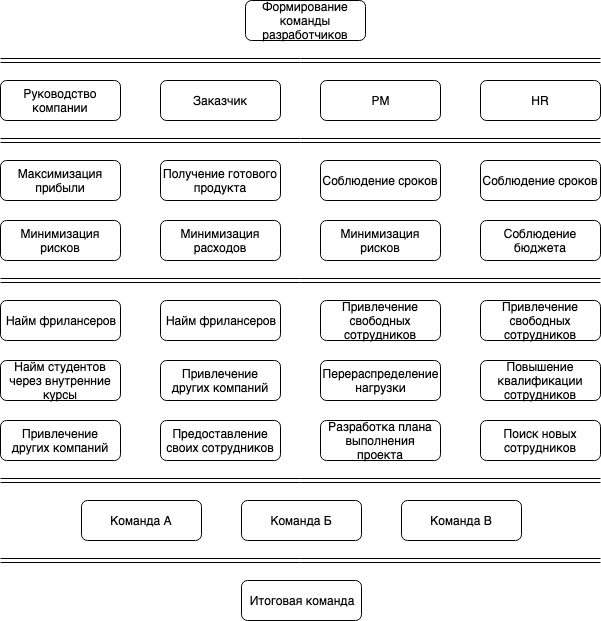
\includegraphics[width=\textwidth]{process}
  \caption{Иерархия прямого процесса формирования команды}
  \label{fig:process}
\end{figure}

При этом $I^i$, $i=\overline{1,6}$ множества элементов $i$-го уровня иерархии. 

На уровне I располагается фокус (главная цель) анализа --- формирование команды разработчиков ($I^1=\{I_1^1\}$). 
Уровень ІІ включает акторов, которые могут влиять на формирование команды. Множество акторов $I^2=\{I^2_j,j=\overline{1,6}\}$ , $j$ --- номер актора. Таким образом, 1 – руководство компании, 2 – заказчик, 3 – менеджер проекта, 4 – кадровый отдел. 
Цели, которые преследуют акторы, составляют ІІІ уровень. Множество целей акторов $I^3=\{I^3_{j,k},j=\overline{1,6},k=\overline{1,t_j}\}$, $k$ --- номер цели $j$-го актора, $t_j$ --- количество целей $j$-го актора. 
Уровень IV включает политики акторов по достижению своих целей. Множество политик акторов $I^4=\{I^4_{j,l},j=\overline{1,6},l=\overline{1,p_j}\}$, $l$ --- номер политики $j$-го актора, $p_j$ --- количество политик $j$-го  актора. 
На уровне V иерархии располагаются исследовательские сценарии $I^5\{I^5_\alpha,\alpha=\overline{1,3}\}$. 
А обобщенный сценарий представляет собой VI уровень $I^6=\{I_1^6\}$.

Проведём парные сравнения элементов одного уровня относительно их действия (весомости, интенсивности) на общую для них характеристику высшего уровня. Также рассчитаем векторы приоритетов и нормализованные векторы приоритетов. После чего рассчитаем для каждой матрицы векторы приоритетов и степени согласованности элементов матриц по формуле:
\[
	CR=\frac{CI}{CIS}
\]
\begin{description}
	\item[где] $CI$ --- индекс согласованности;
	\item $CIS$ --- стохастический коэффициент согласованности матрицы.
\end{description}

Индекс согласованности равен:
\[
	CI=\frac{\lambda_{\max}-n}{n-1}
\]
\begin{description}
	\item[где] $\lambda_{\max}$ --- собственный вектор;
	\item $n$ --- порядок матрицы.
\end{description}

Стохастический коэффициент согласованности матрицы равен:
\[
	CIS=\frac{1.98 \cdot (n-2)}{n}
\]
\begin{description}
	\item[где] $n$ --- порядок матрицы.
\end{description}

% layer 1

Матрица попарного сравнения воздействия акторов на процесс формирования команды:
\[
	A^2 = 
		\begin{array}{c|cccc}
			& I^2_1 & I^2_2 & I^2_3 & I^2_4 \\ \hline
			I^2_1 & 1 & 1.0907 & 3,0880 & 2.2374 \\
			I^2_2 & 0.9168 & 1 & 2,9397 & 0.4923 \\
			I^2_3 & 0.3238 & 0.3401 & 1 & 0.5528 \\
			I^2_4 & 0.4469 & 2.0309 & 1.8087 & 1
		\end{array},
	\textup{НВП}=
		\begin{array}{c}
			0.3801 \\
			0.2462 \\
			0.1139 \\
			0.2596
		\end{array},
	\textup{ОС}=\frac{0.798}{0.9}=0.0886.
\]

% layer 2

Матрица весов целей актора <<руководство компании>>:
\[
	A^3 = 
		\begin{array}{c|cc}
			& I^3_{1,1} & I^3_{1,2} \\ \hline
			I^3_{1,1} & 1 & 2.3530 \\
			I^3_{1,2} & 0.4249 & 1 
		\end{array},
	\textup{НВП}=
		\begin{array}{c}
			0.7017 \\
			0.2982
		\end{array}.
\]

Матрица весов целей актора <<заказчик>>:
\[
	A^3 = 
		\begin{array}{c|cc}
			& I^3_{2,1} & I^3_{2,2} \\ \hline
			I^3_{2,1} & 1 & 2.2575 \\
			I^3_{2,2} & 0.4429 & 1 
		\end{array},
	\textup{НВП}=
		\begin{array}{c}
			0.6930 \\
			0.3069
		\end{array}.
\]

Матрица весов целей актора <<PM>>:
\[
	A^3 = 
		\begin{array}{c|cc}
			& I^3_{3,1} & I^3_{3,2} \\ \hline
			I^3_{3,1} & 1 & 2.7861 \\
			I^3_{3,2} & 0.3589 & 1 
		\end{array},
	\textup{НВП}=
		\begin{array}{c}
			0.7358 \\
			0.2641
		\end{array}.
\]

Матрица весов целей актора <<HR>>:
\[
	A^3 = 
		\begin{array}{c|cc}
			& I^3_{4,1} & I^3_{4,2} \\ \hline
			I^3_{4,1} & 1 & 1.4069 \\
			I^3_{4,2} & 0.7107 & 1 
		\end{array},
	\textup{НВП}=
		\begin{array}{c}
			0.5845 \\
			0.4154
		\end{array}.
\]

Приоритеты альтернативных сценариев имеют такие значения:
\begin{align*}
	I^3_{1,1}=0.1754, I^3_{1,2}=0.0745, \\
	I^3_{2,1}=0.1732, I^3_{2,2}=0.0767, \\
	I^3_{3,1}=0.1839, I^3_{3,2}=0.0660, \\
	I^4_{4,1}=0.1461, I^3_{4,2}=0.1038. \\
\end{align*}

Далее приведены матрицы сравнения весомостей политик акторов по достижения их целей.

% layer 4 

Весомости политик руководства компании в максимизации прибыли.
\[
	A^4 = 
		\begin{array}{c|ccc}
			& I^4_{1,1} & I^4_{1,2} & I^4_{1,3} \\ \hline
			I^4_{1,1} & 1 & 2.5094 & 2.7377 \\
			I^4_{1,2} & 0.3984 & 1 & 0.9739 \\
			I^4_{1,3} & 0.3652 & 1.0267 & 1 
		\end{array},
	\textup{НВП}=
		\begin{array}{c}
			0.5672 \\
			0.2176 \\
			0.2151
		\end{array},
	\textup{ОС}=\frac{0.0007}{0.58}=0.0012.
\]

Весомости политик руководства компании в минимизации затрат.
\[
	A^4 = 
		\begin{array}{c|ccc}
			& I^4_{1,1} & I^4_{1,2} & I^4_{1,3} \\ \hline
			I^4_{1,1} & 1 & 3.7741 & 2.6959 \\
			I^4_{1,2} & 0.6240 & 1 & 0.5360 \\
			I^4_{1,3} & 0.3709 & 1.8656 & 1 
		\end{array},
	\textup{НВП}=
		\begin{array}{c}
			0.6064 \\
			0.1460 \\
			0.2475
		\end{array},
	\textup{ОС}=\frac{0.0045}{0.58}=0.0079.
\]

Весомости политик заказчика в получении готового продукта.
\[
	A^4 = 
		\begin{array}{c|ccc}
			& I^4_{2,1} & I^4_{2,2} & I^4_{2,3} \\ \hline
			I^4_{2,1} & 1 & 2.6949 & 3.2345 \\
			I^4_{2,2} & 0.3710 & 1 & 2.5331 \\
			I^4_{2,3} & 0.3091 & 0.3947 & 1 
		\end{array},
	\textup{НВП}=
		\begin{array}{c}
			0.5824 \\
			0.2772 \\
			0.1403
		\end{array},
	\textup{ОС}=\frac{0.0311}{0.58}=0.0537.
\]

Весомости политик заказчика в минимизации расходов.
\[
	A^4 = 
		\begin{array}{c|ccc}
			& I^4_{2,1} & I^4_{2,2} & I^4_{2,3} \\ \hline
			I^4_{2,1} & 1 & 4.9617 & 4.7641 \\
			I^4_{2,2} & 0.2015 & 1 & 0.4532 \\
			I^4_{2,3} & 0.2099 & 0.2131	1 
		\end{array},
	\textup{НВП}=
		\begin{array}{c}
			0.7010 \\
			0.1100 \\
			0.1889
		\end{array},
	\textup{ОС}=\frac{0.0314}{0.58}=0.0542.
\]

Весомости политик менеджера в соблюдении сроков.
\[
	A^4 = 
		\begin{array}{c|ccc}
			& I^4_{3,1} & I^4_{3,2} & I^4_{3,3} \\ \hline
			I^4_{3,1} & 1 & 0.1738 & 0.9739 \\
			I^4_{3,2} & 5.7533 & 1 & 4.5723 \\
			I^4_{3,3} & 0.2130 & 0.2187	1 
		\end{array},
	\textup{НВП}=
		\begin{array}{c}
			0.1337 \\
			0.7192 \\
			0.1469
		\end{array},
	\textup{ОС}=\frac{0.0022}{0.58}=0.0039.
\]

Весомости политик менеджера в минимизации рисков.
\[
	A^4 = 
		\begin{array}{c|ccc}
			& I^4_{3,1} & I^4_{3,2} & I^4_{3,3} \\ \hline
			I^4_{3,1} & 1 & 1.7580 & 3.7741 \\
			I^4_{3,2} & 0.5688 & 1 & 2.8397 \\
			I^4_{3,3} & 0.2649 & 0.3521 & 1 
		\end{array},
	\textup{НВП}=
		\begin{array}{c}
			0.5359 \\
			0.3346 \\
			0.1293
		\end{array},
	\textup{ОС}=\frac{0.0043}{0.58}=0.0075.
\]

Весомости политик отдела кадров в соблюдении сроков.
\[
	A^4 = 
		\begin{array}{c|ccc}
			& I^4_{4,1} & I^4_{4,2} & I^4_{4,3} \\ \hline
			I^4_{4,1} & 1 & 2.7244 & 1.7580 \\
			I^4_{4,2} & 0.3670 & 1 & 0.9739 \\
			I^4_{4,3} & 0.5688 & 1.0267 & 1 
		\end{array},
	\textup{НВП}=
		\begin{array}{c}
			0.5216 \\
			0.2196 \\
			0.2586
		\end{array},
	\textup{ОС}=\frac{0.0094}{0.58}=0.0162.
\]

Весомости политик отдела кадров в соблюдении бюджета.
\[
	A^4 = 
		\begin{array}{c|ccc}
			& I^4_{4,1} & I^4_{4,2} & I^4_{4,3} \\ \hline
			I^4_{4,1} & 1 3.7741 & 2.8397 \\
			I^4_{4,2} & 0.2649 & 1 & 2.0213 \\
			I^4_{4,3} & 0.3521 & 0.4947 & 1 
		\end{array},
	\textup{НВП}=
		\begin{array}{c}
			0.6166 \\
			0.2271 \\
			0.1562
		\end{array},
	\textup{ОС}=\frac{0.0547}{0.58}=0.0943.
\]

Приоритеты альтернативных сценариев имеют такие значения:
\begin{align*}
	I^4_{1,1}=0.1467, I^4_{1,2}=0.0454, I^4_{1,3}=0.0578, \\
	I^4_{2,1}=0.1604, I^4_{2,2}=0.0484, I^4_{2,3}=0.0411, \\
	I^4_{3,1}=0.0837, I^4_{3,2}=0.1317, I^4_{3,3}=0.0345, \\
	I^4_{4,1}=0.1422, I^4_{4,2}=0.0558, I^4_{4,3}=0.0518.
\end{align*}

Далее приведены матрицы парных сравнений альтернативных сценариев относительно их влияния на политики акторов.

% layer 5

Весомости сценариев в рамках политики найма фрилансеров:
\[
	A^5 = 
		\begin{array}{c|ccc}
			& I^5_1 & I^5_2 & I^5_3 \\ \hline
			I^5_1 & 1 & 0.7748 & 0.5729 \\
			I^5_2 & 1.2906 & 1 & 0.8607 \\
			I^5_3 & 1.7454 & 1.1617 & 1 
		\end{array},
	\textup{НВП}=
		\begin{array}{c}
			0.2489 \\
			0.3379 \\
			0.4130
		\end{array},
	\textup{ОС}=\frac{0.0012}{0.58}=0.0022.
\]

Весомости сценариев в рамках политики найма студентов через внешние курсы:
\[
	A^5 = 
		\begin{array}{c|ccc}
			& I^5_1 & I^5_2 & I^5_3 \\ \hline
			I^5_1 & 1 & 1.1684 & 2.4899 \\
			I^5_2 & 0.8558 & 1 & 3.5513 \\
			I^5_3 & 0.4016 & 0.2815 & 1 
		\end{array},
	\textup{НВП}=
		\begin{array}{c}
			0.4249 \\
			0.4311 \\
			0.1439
		\end{array},
	\textup{ОС}=\frac{0.0145}{0.58}=0.0250.
\]

Весомости сценариев в рамках политики привлечение других компаний:
\[
	A^5 = 
		\begin{array}{c|ccc}
			& I^5_1 & I^5_2 & I^5_3 \\ \hline
			I^5_1 & 1 & 1.6213 & 2.9605 \\
			I^5_2 & 0.6167 & 1 & 1.5745 \\
			I^5_3 & 0.3377 & 0.6351 & 1 
		\end{array},
	\textup{НВП}=
		\begin{array}{c}
			0.5149 \\
			0.3022 \\
			0.1827
		\end{array},
	\textup{ОС}=\frac{0.0012}{0.58}=0.0021.
\]

Весомости сценариев в рамках политики найма фрилансеров:
\[
	A^5 = 
		\begin{array}{c|ccc}
			& I^5_1 & I^5_2 & I^5_3 \\ \hline
			I^5_1 & 1 & 0.5729 & 3.0474 \\
			I^5_2 & 1.7454 & 1 & 4.2355 \\
			I^5_3 & 0.3281 & 0.2360 & 1 
		\end{array},
	\textup{НВП}=
		\begin{array}{c}
			0.3364 \\
			0.5443 \\
			0.1191
		\end{array},
	\textup{ОС}=\frac{0.0028}{0.58}=0.0049.
\]

Весомости сценариев в рамках политики привлечения других компаний:
\[
	A^5 = 
		\begin{array}{c|ccc}
			& I^5_1 & I^5_2 & I^5_3 \\ \hline
			I^5_1 & 1 & 2.9278 & 4.1463 \\
			I^5_2 & 0.3415 & 1 & 3.2603 \\
			I^5_3 & 0.2411 & 0.3067 & 1 
		\end{array},
	\textup{НВП}=
		\begin{array}{c}
			0.6121 \\
			0.2760 \\
			0.1118
		\end{array},
	\textup{ОС}=\frac{0.0388}{0.58}=0.0670.
\]

Весомости сценариев в рамках политики предоставления своих сотрудников:
\[
	A^5 = 
		\begin{array}{c|ccc}
			& I^5_1 & I^5_2 & I^5_3 \\ \hline
			I^5_1 & 1 & 2.9605 & 2.1259 \\
			I^5_2 & 0.3377 & 1 & 1.1429 \\
			I^5_3 & 0.4703 & 0.8749 & 1 
		\end{array},
	\textup{НВП}=
		\begin{array}{c}
			0.5564 \\
			0.2194 \\
			0.2241
		\end{array},
	\textup{ОС}=\frac{0.0120}{0.58}=0.0207.
\]

Весомости сценариев в рамках политики предоставления свободных сотрудников:
\[
	A^5 = 
		\begin{array}{c|ccc}
			& I^5_{}& I^5_2 & I^5_3 \\ \hline
			I^5_1 & 1 & 1.1524 & 2.8489 \\
			I^5_2 & 0.8677 & 1 & 2.3379 \\
			I^5_3 & 0.3510 & 0.4277 & 1 
		\end{array},
	\textup{НВП}=
		\begin{array}{c}
			0.4526 \\
			0.3855 \\
			0.1618
		\end{array},
	\textup{ОС}=\frac{0.0001}{0.58}=0.0002.
\]

Весомости сценариев в рамках политики перераспределения нагрузки:
\[
	A^5 = 
		\begin{array}{c|ccc}
			& I^5_1 & I^5_2 & I^5_3 \\ \hline
			I^5_1 & 1 & 1.1684 & 3.9881 \\
			I^5_2 & 0.8558 & 1 & 3.2603 \\
			I^5_3 & 0.2507 & 0.3067 & 1 
		\end{array},
	\textup{НВП}=
		\begin{array}{c}
			0.4767 \\
			0.4018 \\
			0.1213
		\end{array},
	\textup{ОС}=\frac{0.0001}{0.58}=0.0002.
\]

Весомости сценариев в рамках политики разработки плана проекта:
\[
	A^5 = 
		\begin{array}{c|ccc}
			& I^5_1 & I^5_2 & I^5_3 \\ \hline
			I^5_, & 1 & 0.9977 & 1.8740 \\
			I^5_2 & 1.0022 & 1 & 0.6893 \\
			I^5_3 & 0.5336 & 1.4505 & 1 
		\end{array},
	\textup{НВП}=
		\begin{array}{c}
			0.4060 \\
			0.2913 \\
			0.3026
		\end{array},
	\textup{ОС}=\frac{0.0563}{0.58}=0.0971.
\]

Весомости сценариев в рамках политики привлечения свободных сотрудников:
\[
	A^5 = 
		\begin{array}{c|ccc}
			& I^5_1 & I^5_2 & I^5_3 \\ \hline
			I^5_1 & 1 & 4.0510 & 2.8489 \\
			I^5_2 & 0.2468 & 1 & 1.5279 \\
			I^5_3 & 0.3510 & 0.6544 & 1 
		\end{array},
	\textup{НВП}=
		\begin{array}{c}
			0.6286 \\
			0.2009 \\
			0.1703
		\end{array},
	\textup{ОС}=\frac{0.0336}{0.58}=0.0579.
\]

Весомости сценариев в рамках политики повышения квалификации сотрудников:
\[
	A^5 = 
		\begin{array}{c|ccc}
			& I^5_1 & I^5_2 & I^5_3 \\ \hline
			I^5_1 & 1 & 2.2806 & 3.8780 \\
			I^5_2 & 0.4384 & 1 & 3.2603 \\
			I^5_3 & 0.2578 & 0.3067 & 1 
		\end{array},
	\textup{НВП}=
		\begin{array}{c}
			0.5706 \\
			0.3108 \\
			0.1184
		\end{array},
	\textup{ОС}=\frac{0.0236}{0.58}=0.0407.
\]

Весомости сценариев в рамках политики поисков новых сотрудников:
\[
	A^5 = 
		\begin{array}{c|ccc}
			& I^5_1 & I^5_2 & I^5_3 \\ \hline
			I^5_1 & 1 & 1.6745 & 4.8116 \\
			I^5_2 & 0.5971 & 1 & 1.6408 \\
			I^5_3 & 0.2078 & 0.6094 & 1 
		\end{array},
	\textup{НВП}=
		\begin{array}{c}
			0.5727 \\
			0.2837 \\
			0.1434
		\end{array},
	\textup{ОС}=\frac{0.0174}{0.58}=0.0301.
\]

Значение степени согласованности для всех матриц меньше критического, что говорит о согласованности параметров.

Приоритеты альтернативных сценариев имеют такие значения:
\begin{description}
	\item $I^5_1=0.4834$ (команда А);
	\item $I^5_2=0.3321$ (команда Б);
	\item $I^5_3=0.1844$ (команда В).
\end{description}

В итоге, сценарий <<Команда А>> является наиболее приемлемой альтернативой. Разработанная политика должна в наибольшей мере следовать данному сценарию.

\subsection{Выводы}

В ходе лабораторной работы был изучен процесс формирования и принятия решения на основе МАИ. Была построена качественная модель проблемы в виде иерархии, определены приоритеты всех элементов иерархии с использованием метода парных сравнений, проверена согласованность суждений и принято решение.

\end{document}
